\documentclass[12pt,a4paper]{article}
\usepackage[utf8]{inputenc}
\usepackage{mathptmx}
\usepackage{graphicx}
\usepackage{float}
\usepackage{hyperref}
\usepackage{url}
\usepackage{csvsimple-l3}

\usepackage{listings}
\usepackage{xcolor}


% --------------------------------------------------------------------
% Code listing setup
% --------------------------------------------------------------------
\definecolor{codegreen}{rgb}{0,0.6,0}
\definecolor{codegray}{rgb}{0.5,0.5,0.5}
\definecolor{codepurple}{rgb}{0.58,0,0.82}
\definecolor{backcolor}{rgb}{0.98,0.98,0.98}

\lstdefinestyle{mystyle}{
   backgroundcolor=\color{backcolor},
   commentstyle=\color{codegreen},
   keywordstyle=\color{magenta},
   numberstyle=\tiny\color{codegray},
   stringstyle=\color{codepurple},
   basicstyle=\ttfamily\scriptsize,
   frame=shadowbox,
   breakatwhitespace=false,
   breaklines=true,
   captionpos=b,
   keepspaces=true,
   numbers=left,
   numbersep=8pt,
   showspaces=false,
   showstringspaces=false,
   showtabs=false,
   tabsize=2
}

\lstset{style=mystyle}


% --------------------------------------------------------------------
% Front page setup (Change this)
% --------------------------------------------------------------------
\newcommand{\HRule}[1]{\rule{\linewidth}{#1}} 	% Horizontal rule

\makeatletter							% Title
\def\printtitle{%						
   {\centering \@title\par}}
\makeatother									

\makeatletter							% Author
\def\printauthor{%					
   {\centering \large \@author}}				
\makeatother							

\title{	\normalsize \textsc{FYS-STK4155 - Applied Data Analysis and Machine Learning} 	% Subtitle
		 	\\[2.0cm]								% 2cm spacing
			\HRule{2pt} \\	[0.5cm]				% Upper rule
			\LARGE \textbf{\uppercase{Project 2}}	% Title
			\HRule{2pt} \\ [0.5cm]		% Lower rule + 0.5cm spacing
         \normalsize November 2021 \\
		}

\author{
		Håkon Muggerud\\
		Diederik van Duuren \\
		Alf Sommer Landsend
      \begin{center}       
         
\includegraphics[width=\textwidth]{UiO.png}
      \end{center}
}

% --------------------------------------------------------------------
% BEGIN DOCUMENT
% --------------------------------------------------------------------
\begin{document}

\thispagestyle{empty}		% Remove page numbering on this page

\printtitle					% Print the title data as defined above
  	\vfill
\printauthor				% Print the author data as defined above
\newpage

\begin{abstract}
    Feed forward neural networks can be used for both regression and classification problems. In this report we tried to predict the surface of the Franke function using a neural network. Using the SGD algorithm we could compare it to the analytical solutions of OLS and ridge regression, and then also to our own neural network using the same SGD. 
\end{abstract}
\newpage

\tableofcontents
\thispagestyle{empty}
\newpage


\section{Introduction}
Artificial neural networks have lately become popular partly because of increased computational capacity. Feed-forward neural networks can among other things be used for classification and regression \cite{jain1996}. In this project we will develop our own feed-forward neural network and study both classification and regression. We will compare the results with the results from our own ordinary least squares and logistic regression code and with results obtained with Scikit-Learn.


\section{Methods}

    \subsection{Stochastic gradient descent}

    In this part of the project we started by replacing in our standard ordinary least squares and Ridge regression codes from project 1 the matrix inversion algorithm with our own stochastic gradient descent (SGD) code.

    \lstinputlisting{scr/SGD.txt}

    We tried to predict values that were calculated by means of the Franke function with noise added. For this we used polynomials of degree 10. For ordinary least squares regression we tried different values of the learning rate in order to find the learning rate that gave the lowest MSE value and the highest R2 value. For Ridge regression we made a grid search to find the hyper-parameter $\lambda$ and the learning rate that gave the highest R2 value.
    
    \subsection{Neural network code}
    
    We wrote our own feed forward neural network code. As activation function for the hidden layer we used the sigmoid function in this part of the project. The activations of the final output layer were scaled. The weights and biases were initialized, using the standard normal distribution. In order to train the network we used stochastic gradient descent.
    We studied the Franke function. The results obtained with our neural network were compared to those obtained with ordinary least squares regression and Scikit-learn.
    \subsection{Testing different activation functions}
    
    We tried to replace the sigmoid activation function with the RELU activation function  in the hidden layer of our own neural network. We also replaced the RELU activation function with the sigmoid activation function in the hidden layers of the Scikit-learn MLP-regressor.
    
    
\newpage
\section{Results}
    \subsection{Stochastic gradient descent}

    \begin{figure}[H]
        \centering
        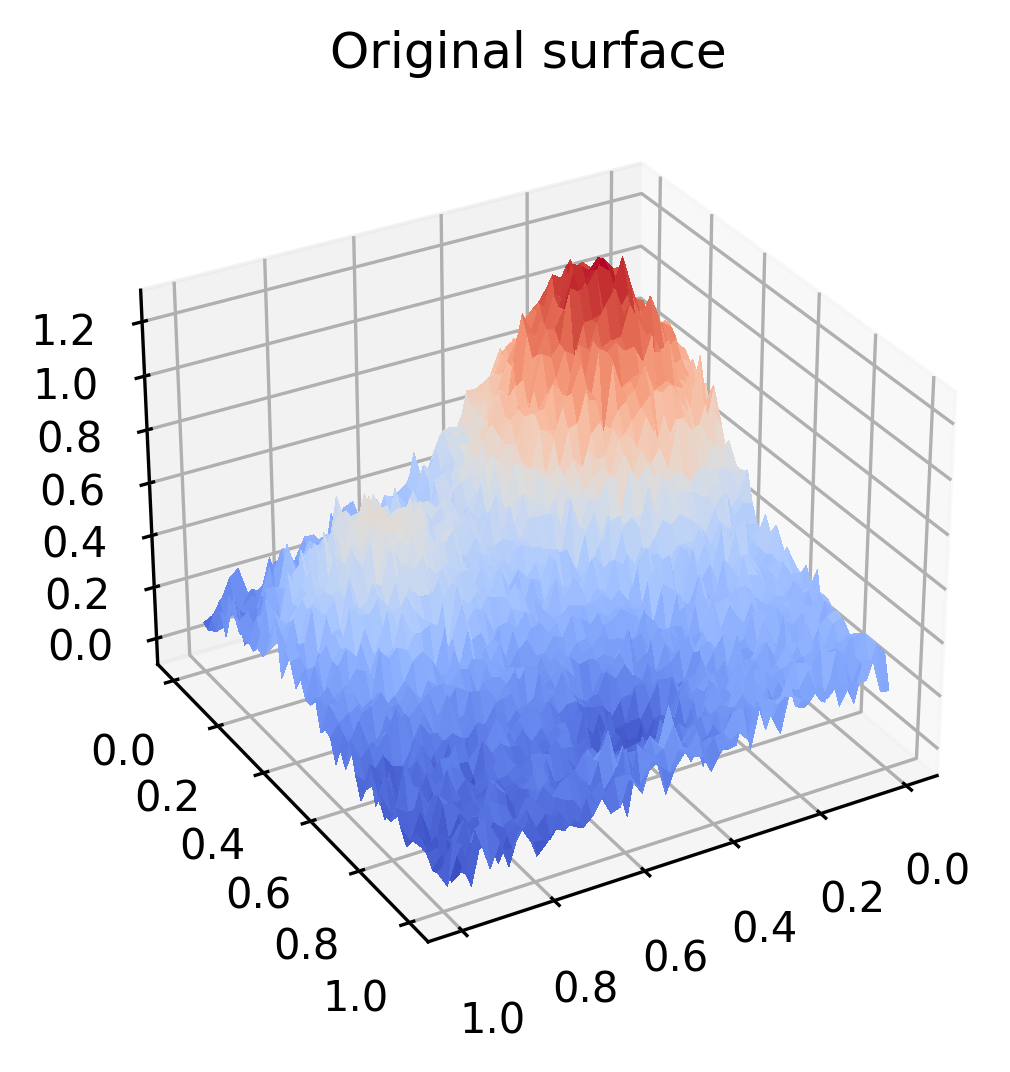
\includegraphics[width=0.5\textwidth]{figures/franke_original.png}
        \caption{The original surface of the Franke function}
        \label{fig:original_franke}
    \end{figure}

    Our models were trained to predict the Franke function showed in figure \ref{fig:original_franke}. Figure \ref{fig:SGD_eta_graph} shows the test mean squared error and test R2 respectively as a function of the logarithm of the learning rate. As one can see the learning rate must have a certain size.

    \begin{figure}[H]
        \centering
        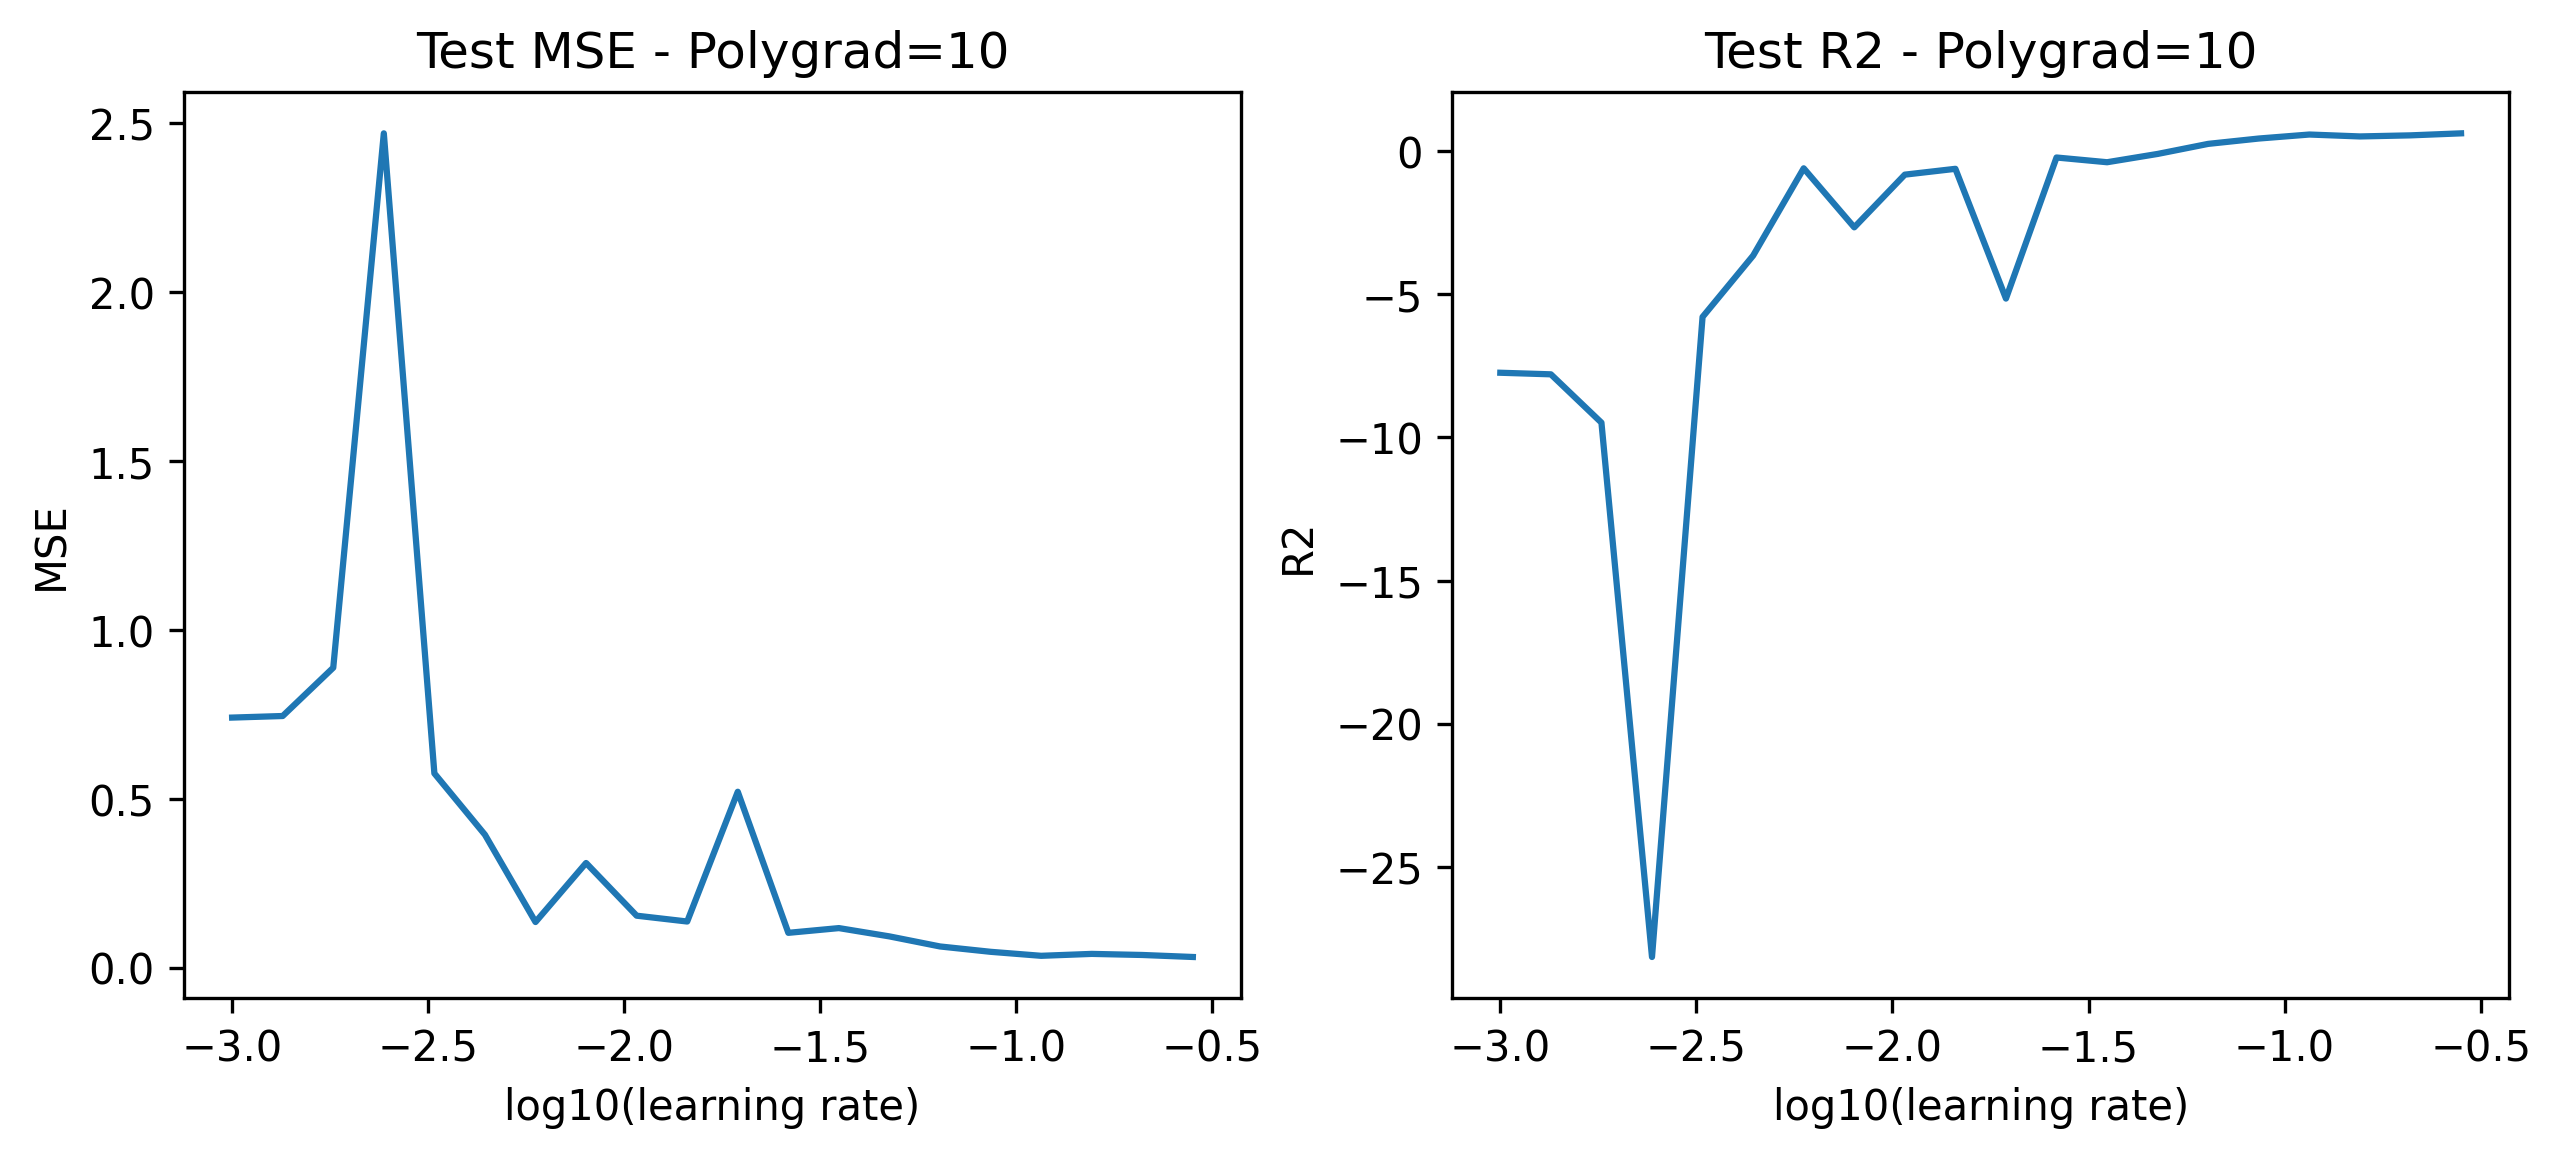
\includegraphics[width=\textwidth]{figures/sgd_linreg_constant_eval.png}
        \caption{SGD for linear regression as a function of learning rate}
        \label{fig:SGD_eta_graph}
    \end{figure}

    The grid search in figure \ref{fig:grid} shows that the best value of $\lambda$ is 0.0001, which is as low as it can be in this grid search, and the best learning rate is 0.1. We wanted to look at values larger than 0.1 for the learning rate, but the function would diverge at a rate around 0.3.

    \begin{figure}[H]
        \centering
        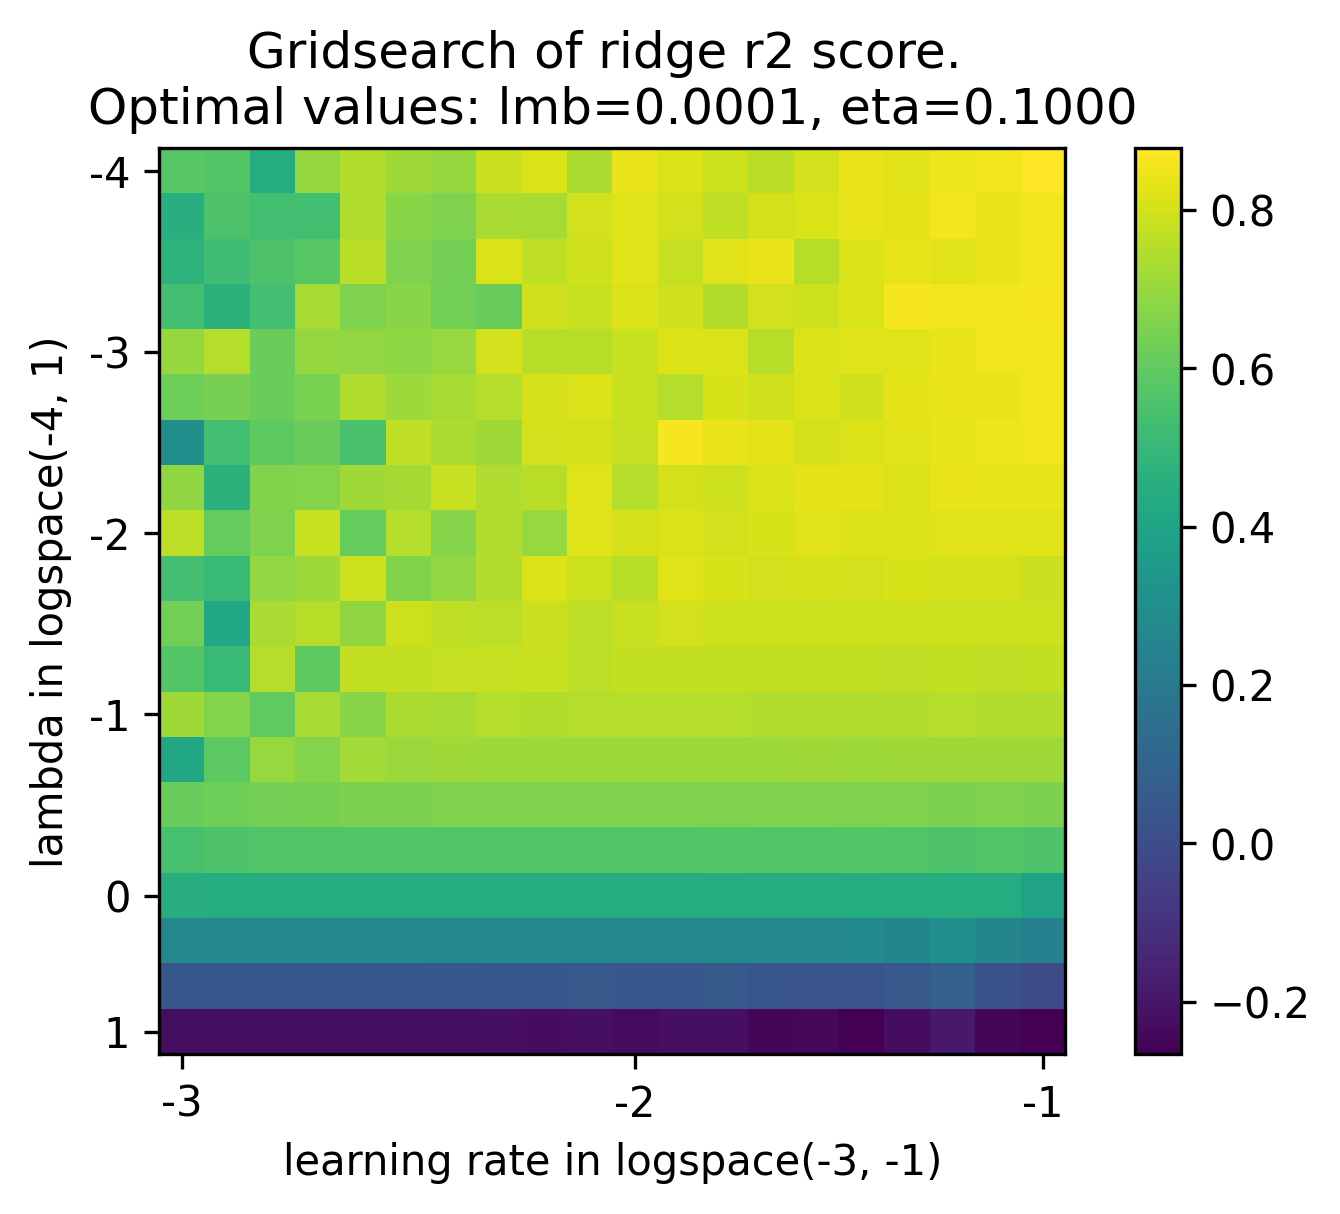
\includegraphics[width=0.5\textwidth]{figures/gridsearch_eta_lmb_ridge.png}
        \caption{Gridsearch of ridge regression  $\lambda$ and the learning rate}
        \label{fig:grid}
    \end{figure}

    For ordinary least squares regression we found that the SGD code gave higher MSE (0.010) and lower R2 value (0.884) than the matrix inversion algorithm (MSE 0.005 and R2 0.941). The learning rate for the SGD was 0.25.

    \begin{figure}[H]
        \centering
        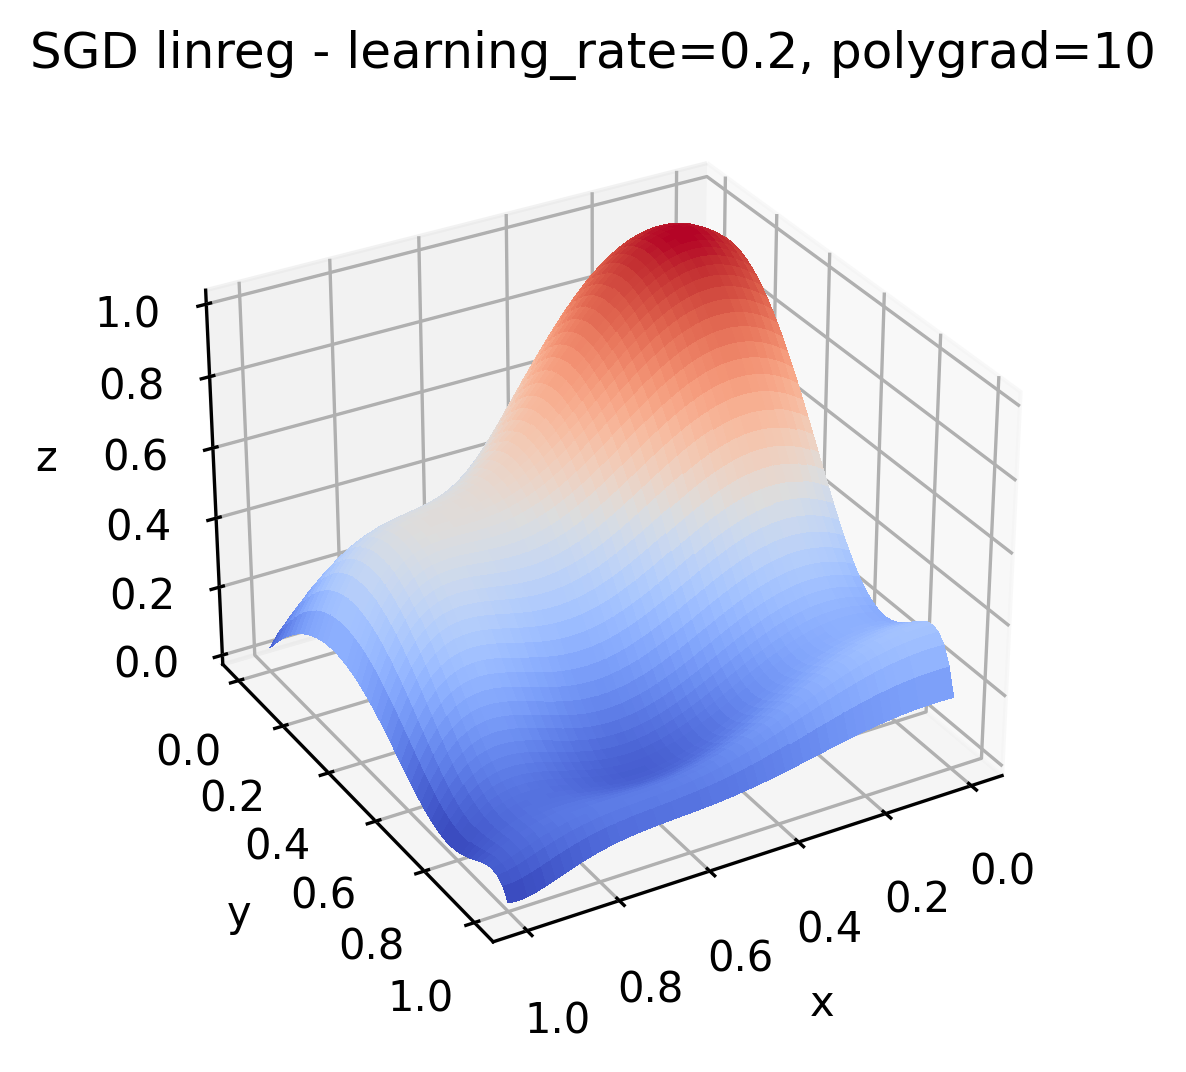
\includegraphics[width=0.5\textwidth]{figures/sgd_linreg_constant_surface.png}
        \caption{SGD applied to linear regression to predict the Franke surface}
        \label{fig:surface_OLS_SGD}
    \end{figure}

    As for ordinary least squares regression we also found for Rigde regression that the SGD code gave higher MSE (0.009) and lower R2 value (0.890) than the matrix inversion algorithm (MSE 0.005 and R2 0.943). The results for Ridge regression are marginally better than those for ordinary least squares. The learning rate for the SGD was 0.1 and $\lambda$ was 0.0001.

    \subsection{Franke surface predictions}

    \begin{figure}[H]
        \centering
        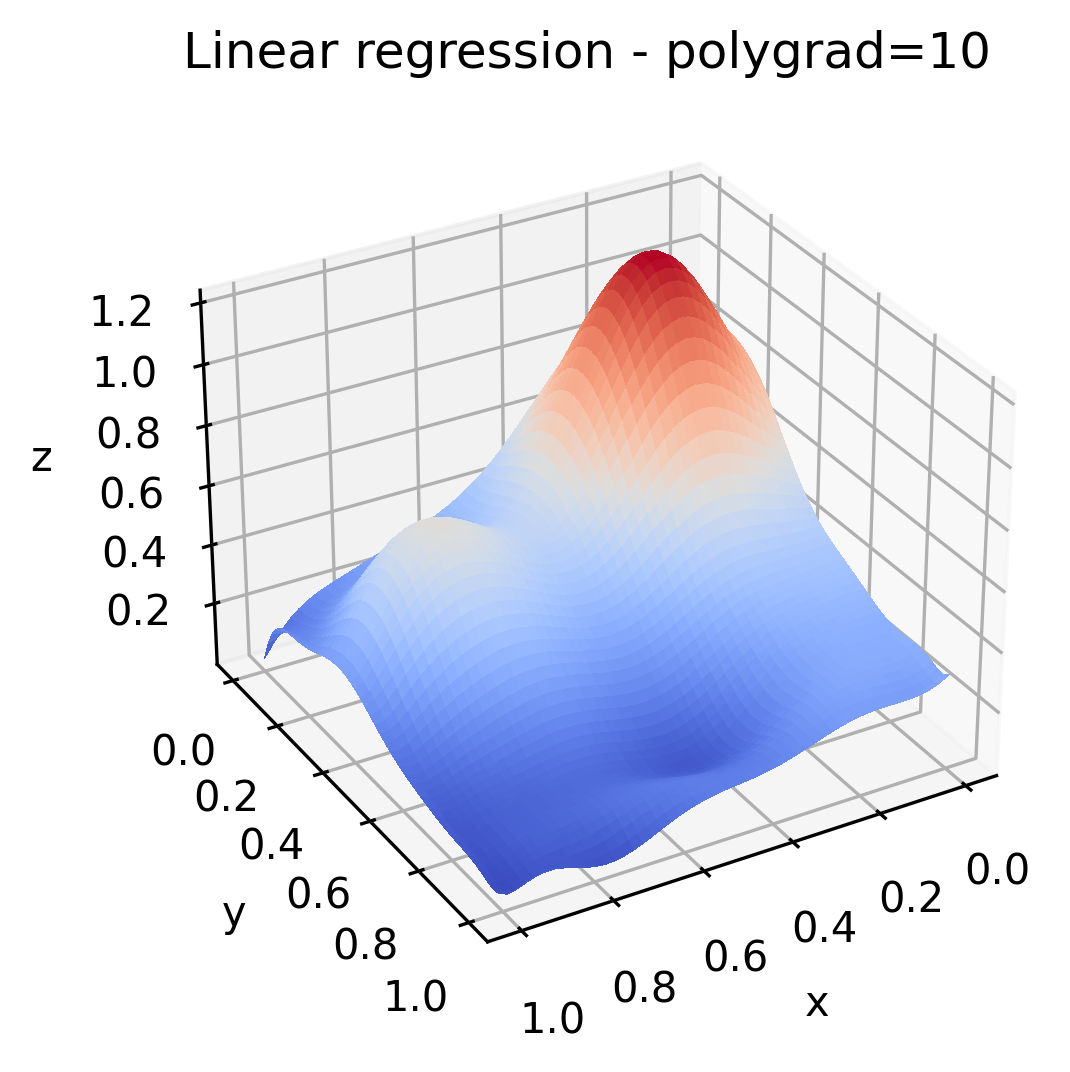
\includegraphics[width=0.5\textwidth]{figures/franke_linreg_sufrace.png}
        \caption{Prediction of the Franke surface with regular OLS. This gave a test R2-value of 0.955 and a test MSE of 0.003.}
        \label{fig:linreg_surface}
    \end{figure}

    \begin{figure}[H]
        \centering
        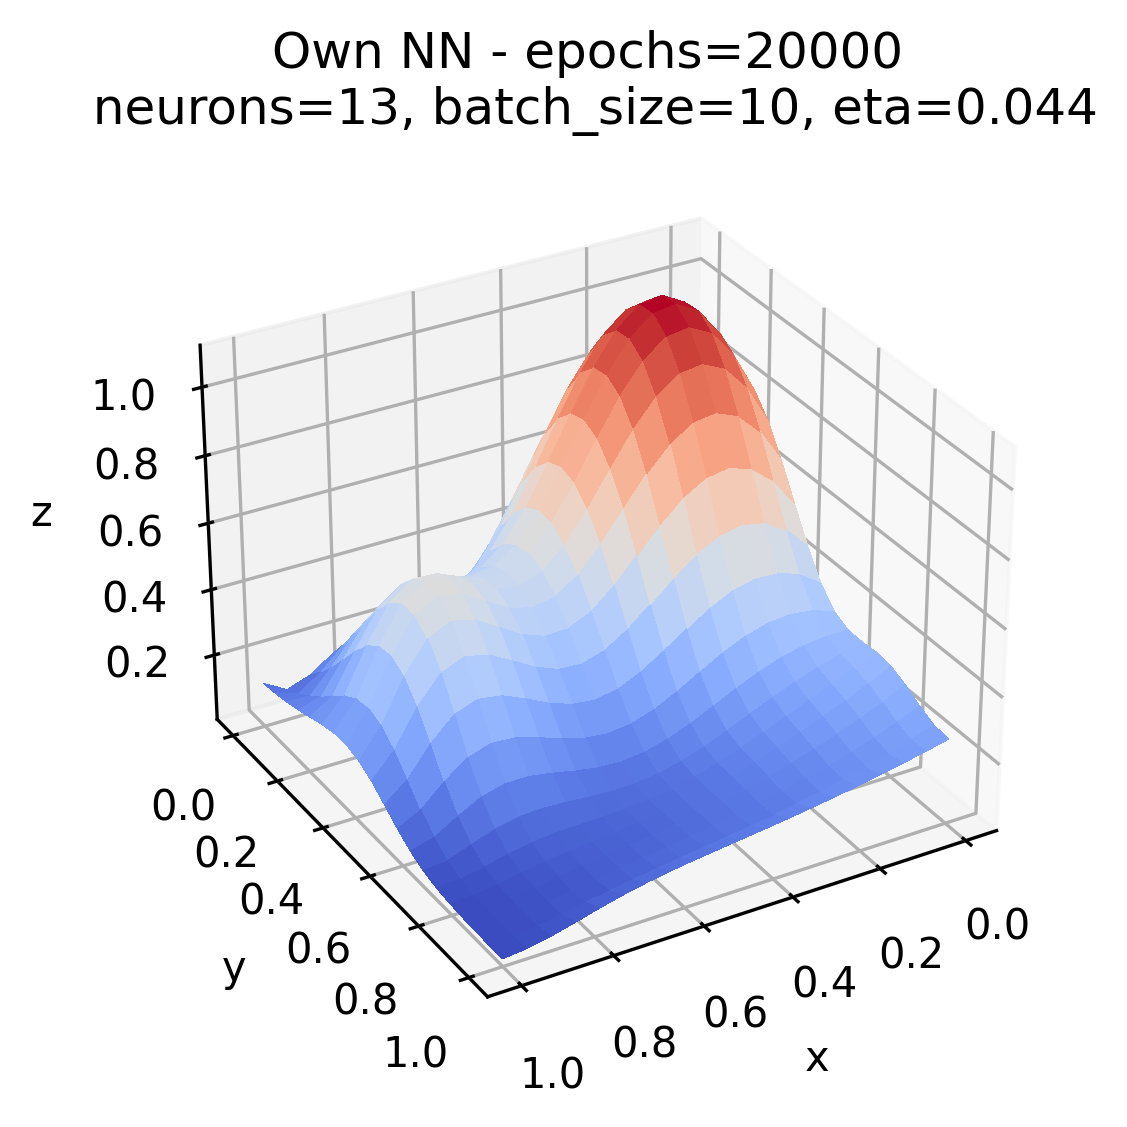
\includegraphics[width=0.5\textwidth]{figures/own_nn_surface1.png}
        \caption{Prediction of the Franke surface with our own neural network. This gave a test R2-value of 0.940 and a test MSE of 0.004.}
        \label{fig:own_nn_surface}
    \end{figure}

    \begin{figure}[H]
        \centering
        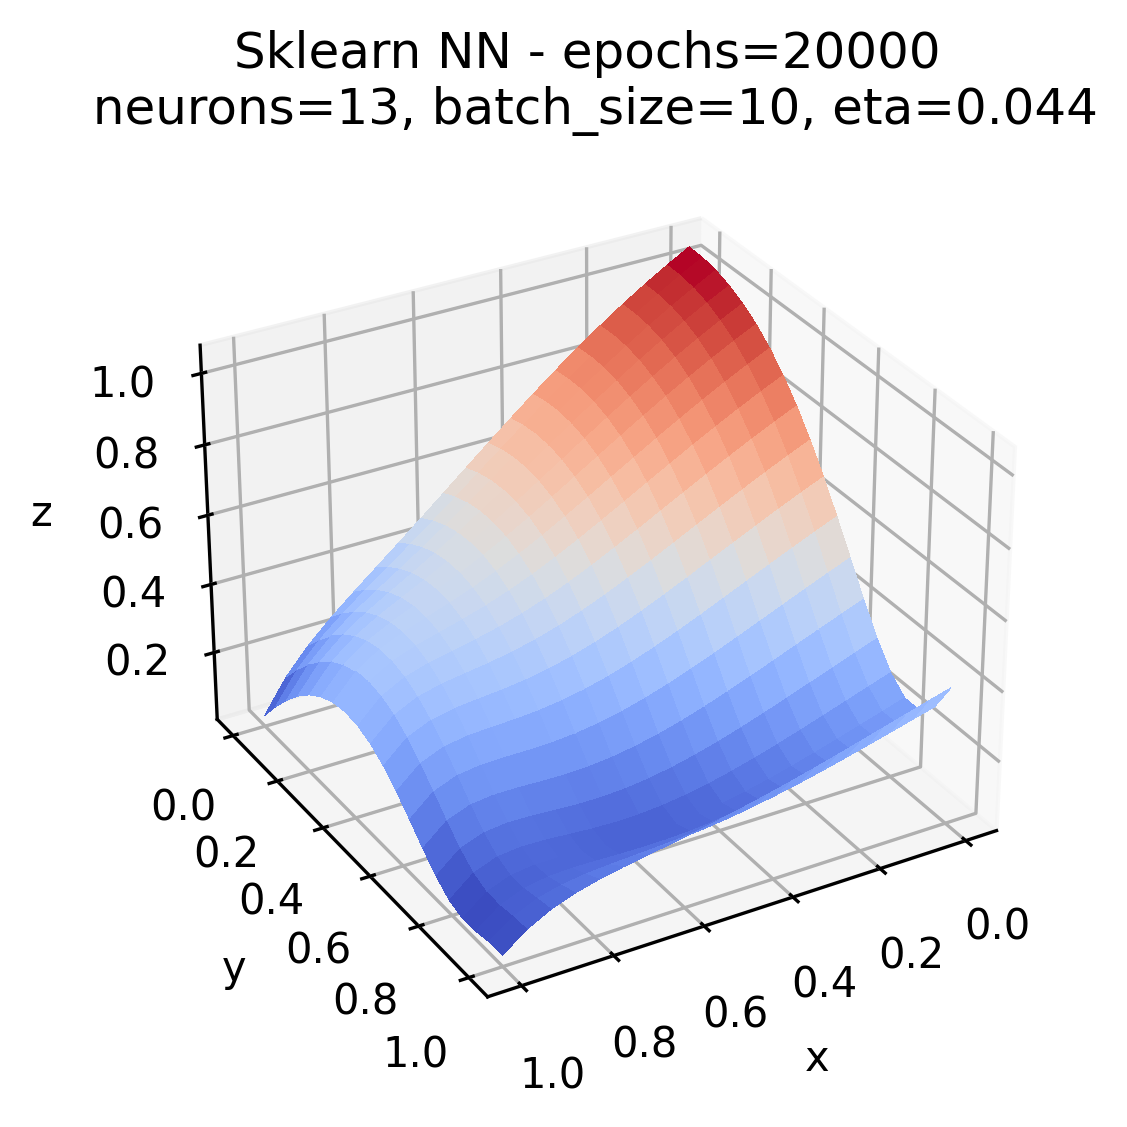
\includegraphics[width=0.5\textwidth]{figures/sklearn_nn_surface1.png}
        \caption{Prediction of the Franke surface with Scikit-Learn NN with the same hyperparameters as figure \ref{fig:own_nn_surface}. This gave a test R2-value of 0.824 and a test MSE of 0.012.}
        \label{fig:nn_sklearn_surf1}
    \end{figure}
    
    \begin{figure}[H]
        \centering
        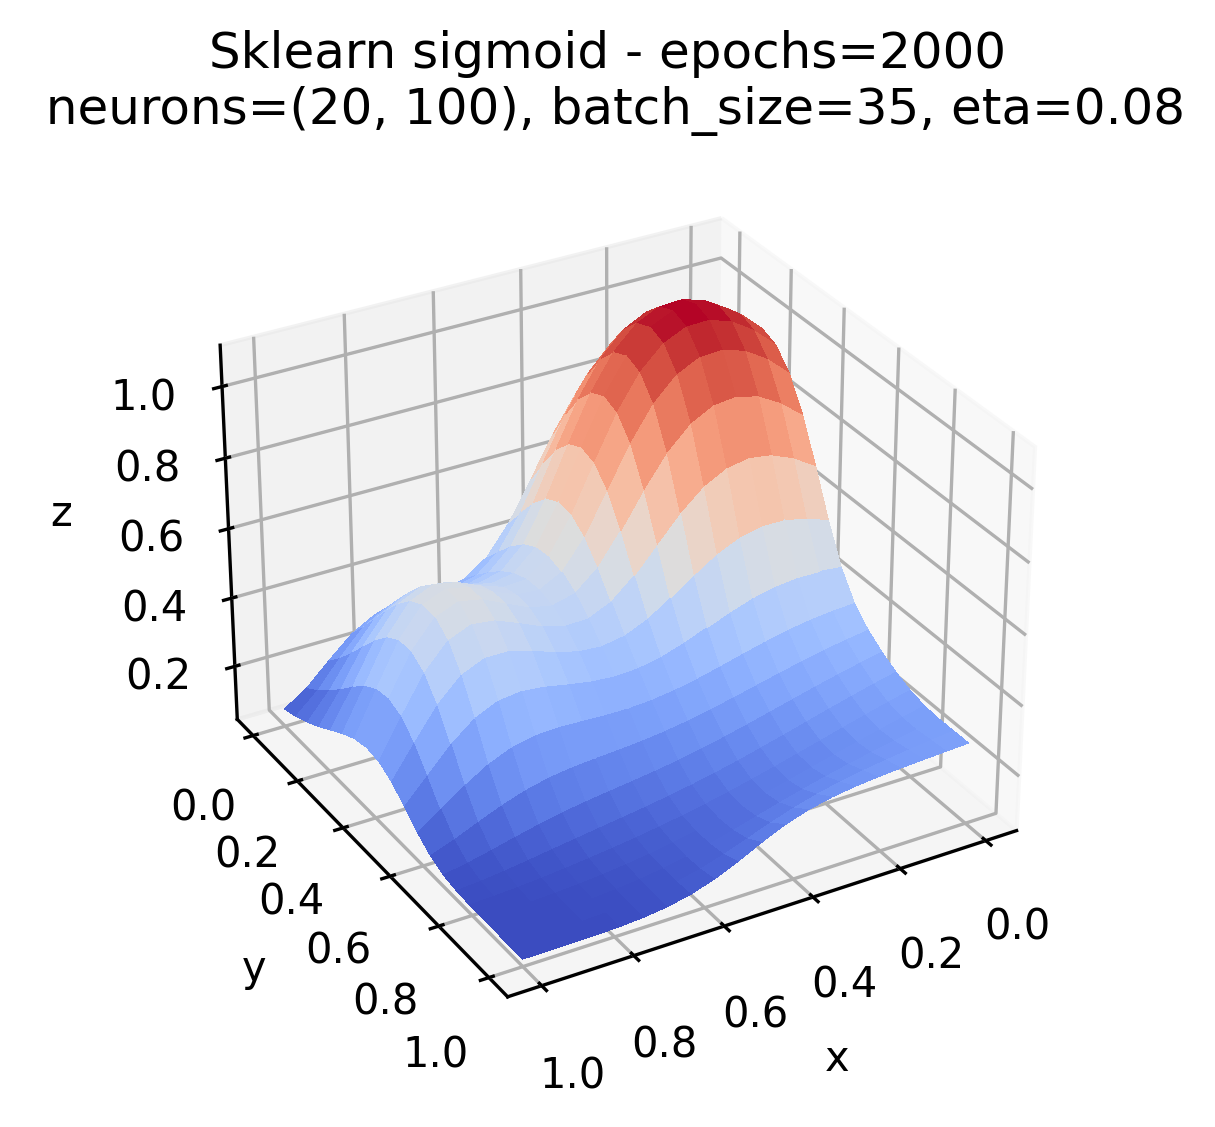
\includegraphics[width=0.5\textwidth]{figures/sklearn_sigmoid.png}
        \caption{Prediction of the Franke surface with Scikit-Learn NN with the sigmoid activation function. This gave a test R2-value of 0.930 and a test MSE of 0.004.}
        \label{fig:nn_sklearn_surf2}
    \end{figure}
    
    \begin{figure}[H]
        \centering
        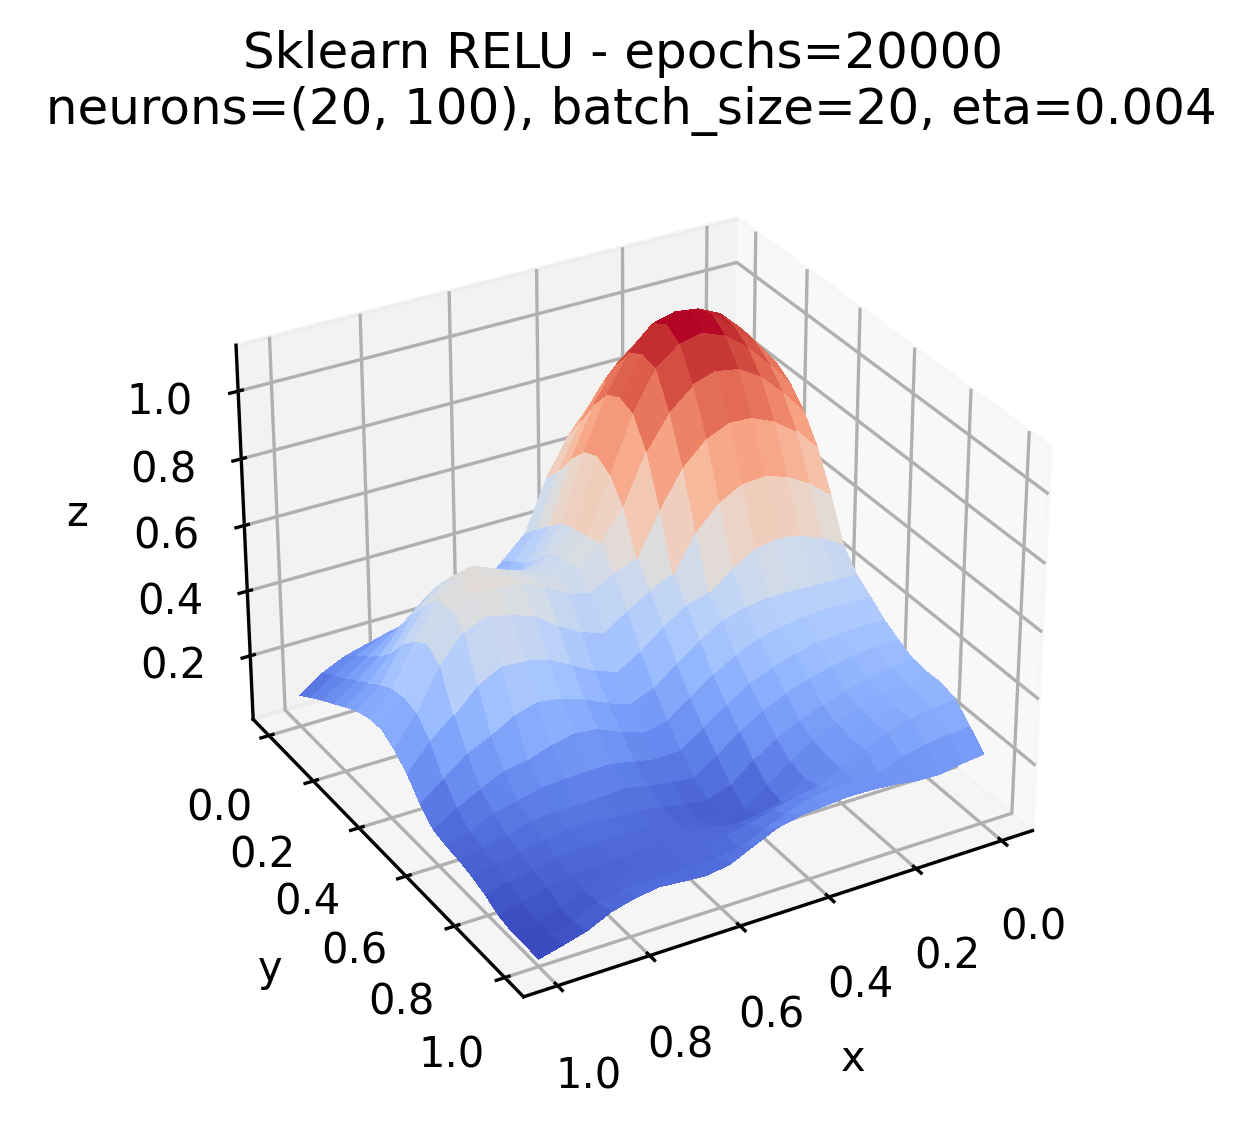
\includegraphics[width=0.5\textwidth]{figures/sklearn_relu.png}
        \caption{Prediction of the Franke surface with Scikit-Learn NN with the RELU activation function. This gave a test R2-value of 0.950 and a test MSE of 0.003.}
        \label{fig:nn_sklearn_surf3}
    \end{figure}
    
    \begin{table}[H]
        \centering
        \csvautotabular{results/ex2_compare}
        \caption{Comparison of the r2 scores of our different models}
        \label{tab:ex2comapare}
    \end{table}


\subsection{Testing different activation functions}

When we replaced the sigmoid activation function with the RELU activation function in the hidden layer of our own neural network and used the network to predict the Franke function, we got an test R2-value of -1497 and an test MSE of 102.1. The graph looked very different form the Franke funktion graph. When the RELU activation function was replaced with the sigmoid activation function in the hidden layers of the Scikit-Learn MLP-regressor, the test R2-value was reduced from 0.950 to 0.931, and the test MSE was increased from 0.00338 to 0.00472.


\section{Discussion}
When we replaced the matrix inversion algorithm with an SGD code our findings for Ridge regression were consistent with those for ordinary least squares regression. In both cases the matrix inversion algorithm gave the best results. The reason for this could be that the SGD code only finds a local minimum.
% Discussion part b remains to be written.
The fact that the R2-value decreased and the MSE increased when the RELU activation function was replaced with the sigmoid activation function in the hidden layers of the Scikit-Learn MLP-regressor, was as one would expect. In general the RELU function performs better than the sigmoid function. 

There could also be some uncertainties regarding this result because we are comparing our own implementation to Scikit-Learn. We didn't use our own RELU fucntion because of issues where our weights diverged and provided results that were not useful. This issue persisted when we were adjusting the network to be used in classification. Logistic regression was not explored in this report.

\section{Conclusion}
When comparing the SGD algorithm to the analytical solutions for OLS and ridge we got our expected results. With such a high feature count the SGD couldn't quite find the global minimum, but it still did a pretty good job at the prediction. As the learning rate increased, the model also performed better. But after a learning rate of about 0.3 the model would diverge. 

When predicting the surface of the Franke fucntion, the best result was achieved with regular OLS. We might have gotten a better result with more tweaking of the hyper parameters, but for this scenario the neural network did not perform better than the analytical solutions, although it only scored 0.005 points lower on the R2 score. 

When we compared the activation functions, the RELU function outperformed the sigmoid functions for Scikit-Learn's implementation. The leaky RELU function could also be explored. 

Our implementation did not work for classification as the weights in our network would diverge when trying to use different activation function for the hidden layers and the output layer. The difference between logistic regression and classification with neural networks could also be explored.

\newpage

\bibliographystyle{unsrt}
\bibliography{ref}

\end{document}